\documentclass[10pt]{beamer}

\usetheme{sidebar}
\usepackage[italian]{babel}
\usepackage[utf8x]{inputenc}
\usepackage {eurosym}
\setbeamercovered{transparent}

%
% The following info should normally be given in you main file:
%
\setbeamertemplate{footline}{
\hfill \begin{center}
 \textbf{Pagina \insertframenumber, di \inserttotalframenumber }
\end{center}

}
\title{Revisione dei requisiti}
\author{Team QuiXoft}
\date{12 Dicembre 2008}


\begin{document}
\transduration{1}

\frame{
	\transsplitverticalin
	\titlepage 
\begin{center}
 
\includegraphics[scale=0.20]{logo.png}
\end{center}
}
\part{Analisi dei requisiti}

\frame{
	\transsplitverticalin
	\partpage }

\section{Analisi dei requisiti}
\subsection{Aggiornamento Analisi dei requisiti}
\frame{
	\frametitle{Analisi dei requisiti}
  \framesubtitle{Aggiornamento Analisi dei requisiti}
  
\begin{itemize}
 \item Eliminazione della segreteria generale
 \item Presidente del CCS e Segreteria didattica hanno le stesse funzioni
 \item I docenti verrano invitati tramite mail ad inserire i propri dati
 \item Vincoli dei docenti devono essere motivati, le preferenze no

\end{itemize}
  \transsplitverticalin
	 }

\part{Specifica tecnica}
\frame{
	\transsplitverticalin
	\partpage }
\section{Specifica tecnica}
\subsection{Descrizione dei pattern}
\frame{
  \frametitle{Specifica tecnica}
  \framesubtitle{Descrizione dei pattern}
  \transsplitverticalin
  }
\subsection{Descrizione dei componenti}
\frame{
 \frametitle{Specifica tecnica}
 \framesubtitle{Descrizione dei componenti}
\begin{Large}\textbf{Diagramma dei componenti}\end{Large}
	\begin{center}
 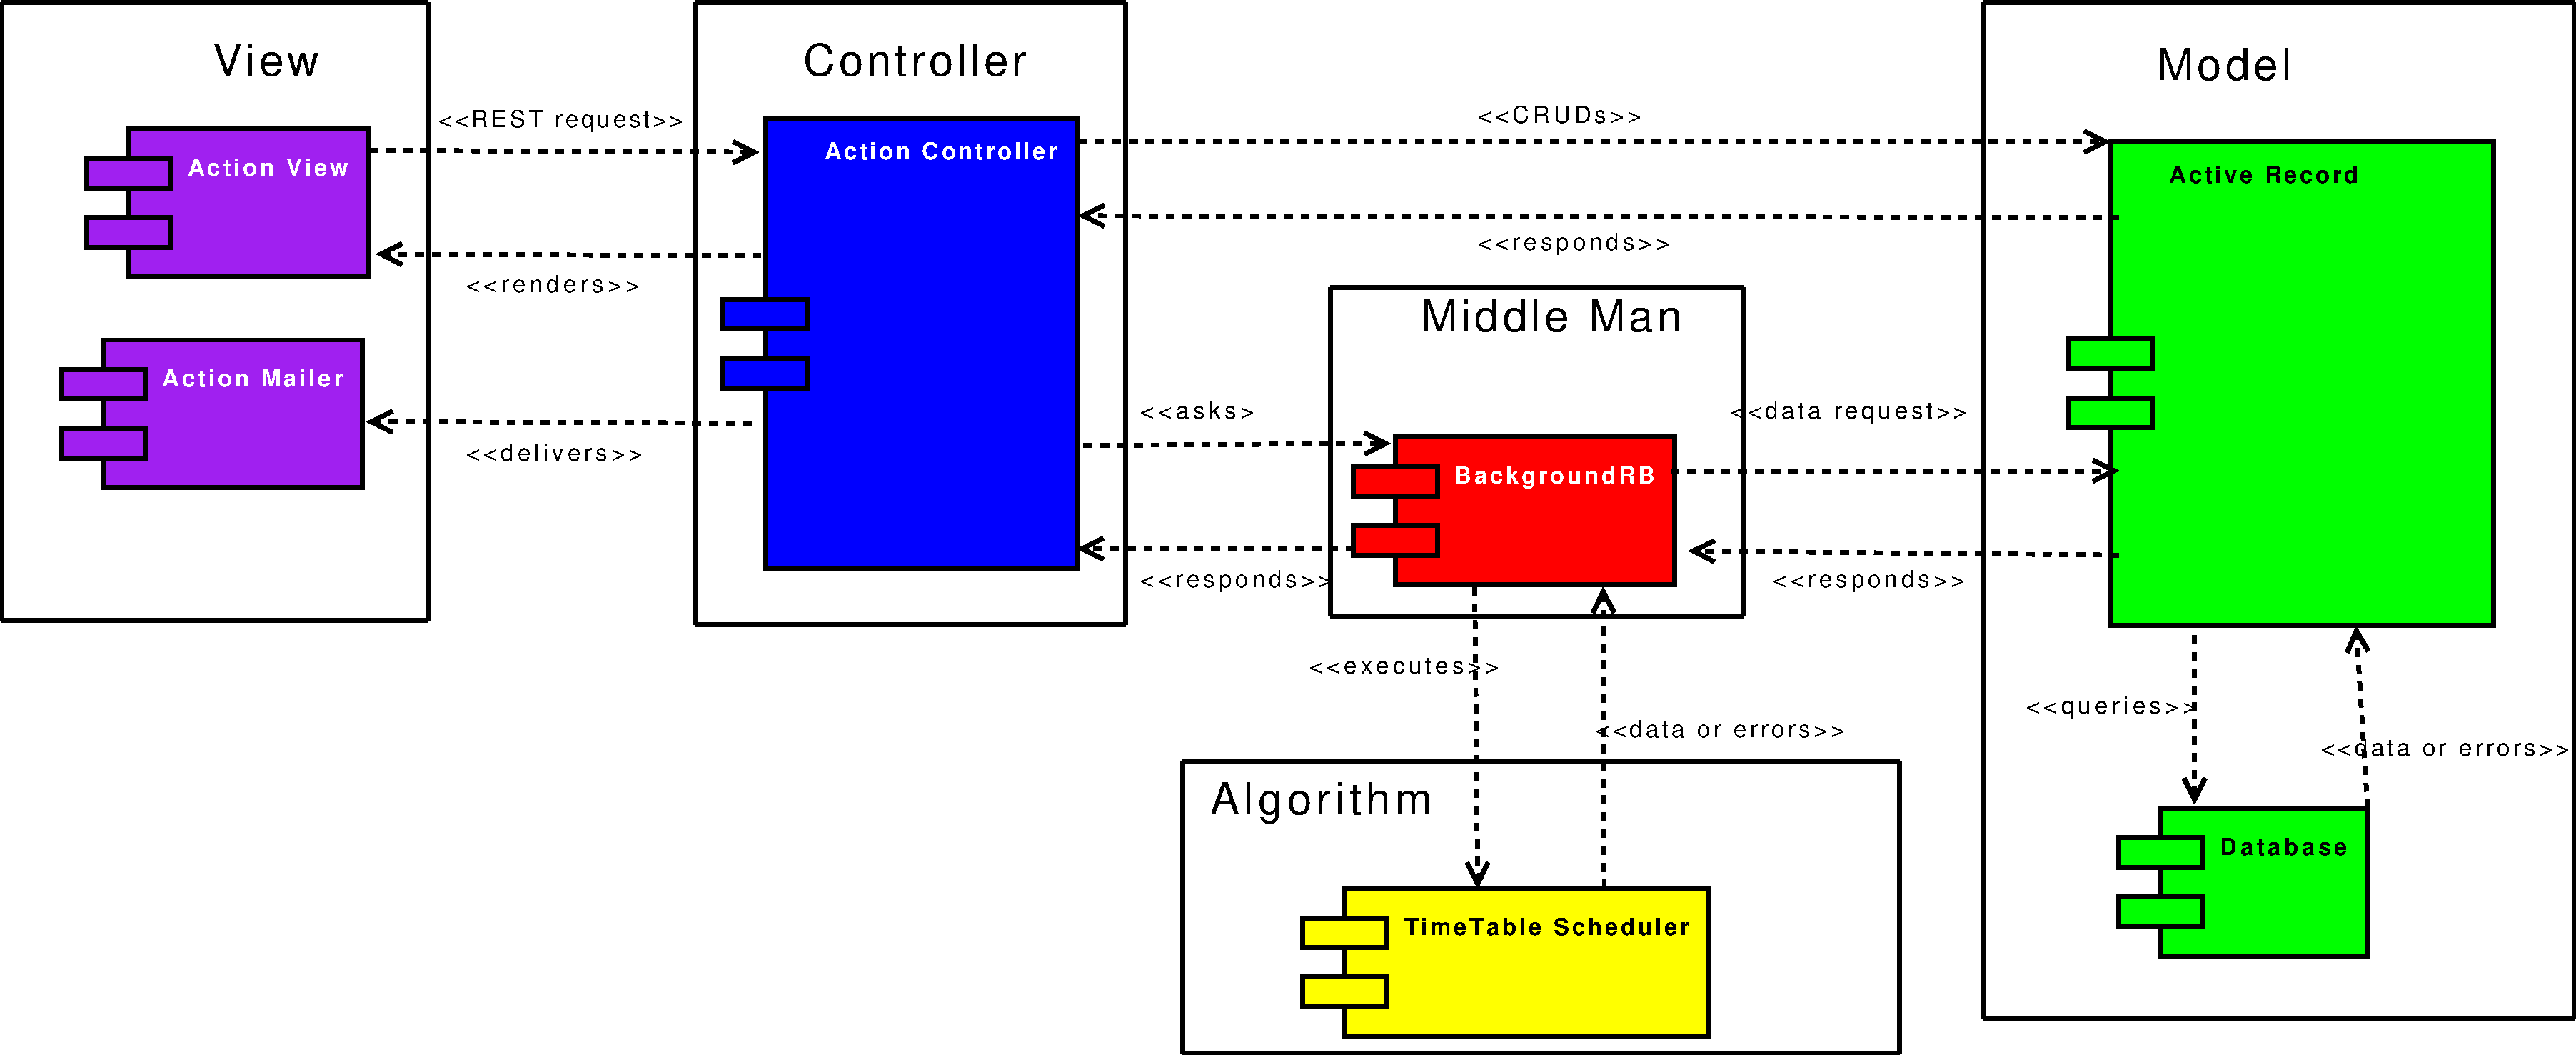
\includegraphics[scale=0.15]{images/diagramma_componenti.pdf}
\end{center}
 \transsplitverticalin
}
\frame{
 \frametitle{Specifica tecnica}
 \framesubtitle{Descrizione dei componenti}
\begin{Large}\textbf{View}\end{Large}
	\begin{center}
 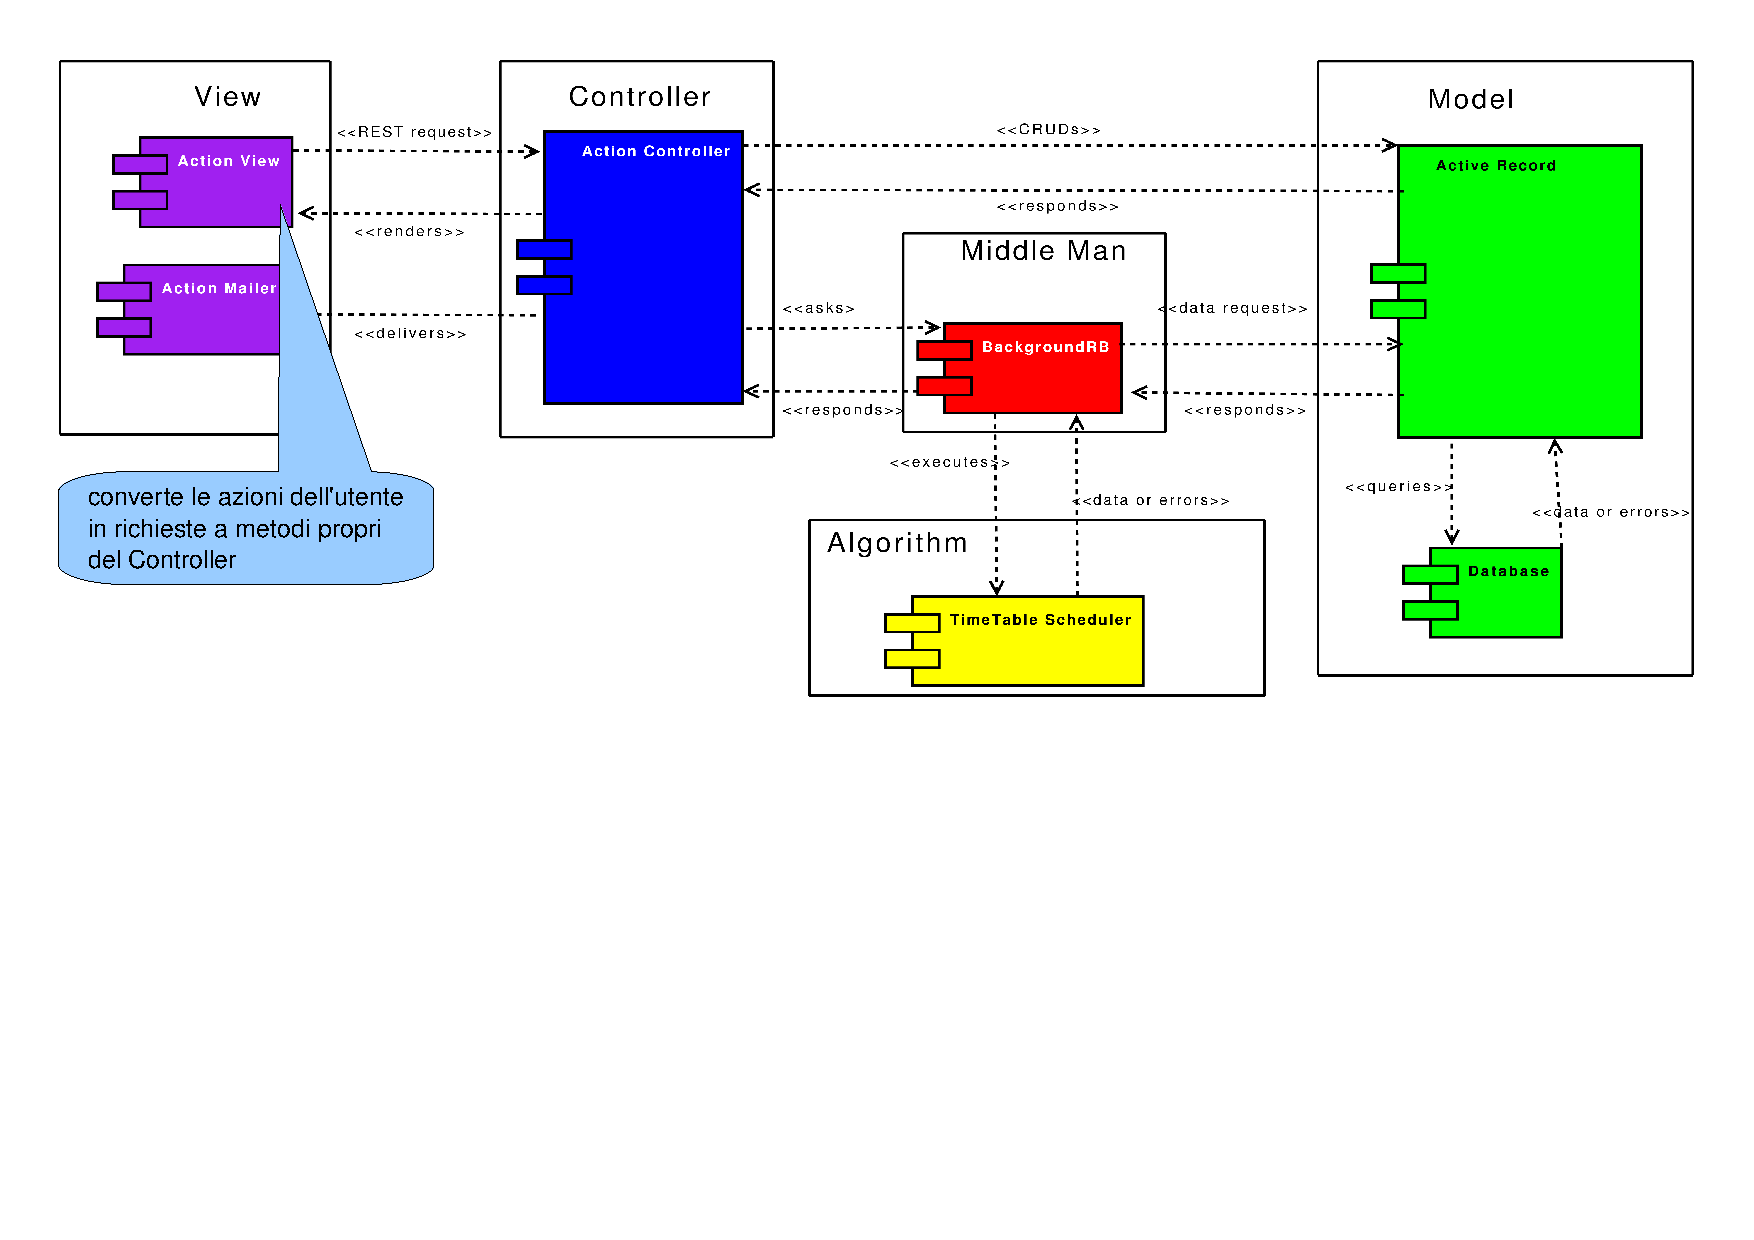
\includegraphics[scale=0.4]{images/diagramma_componenti_view.pdf}
\end{center} \transsplitverticalin
}
\frame{
 \frametitle{Specifica tecnica}
 \framesubtitle{Descrizione dei componenti}
\begin{Large}\textbf{Controller}\end{Large}
	\begin{center}
 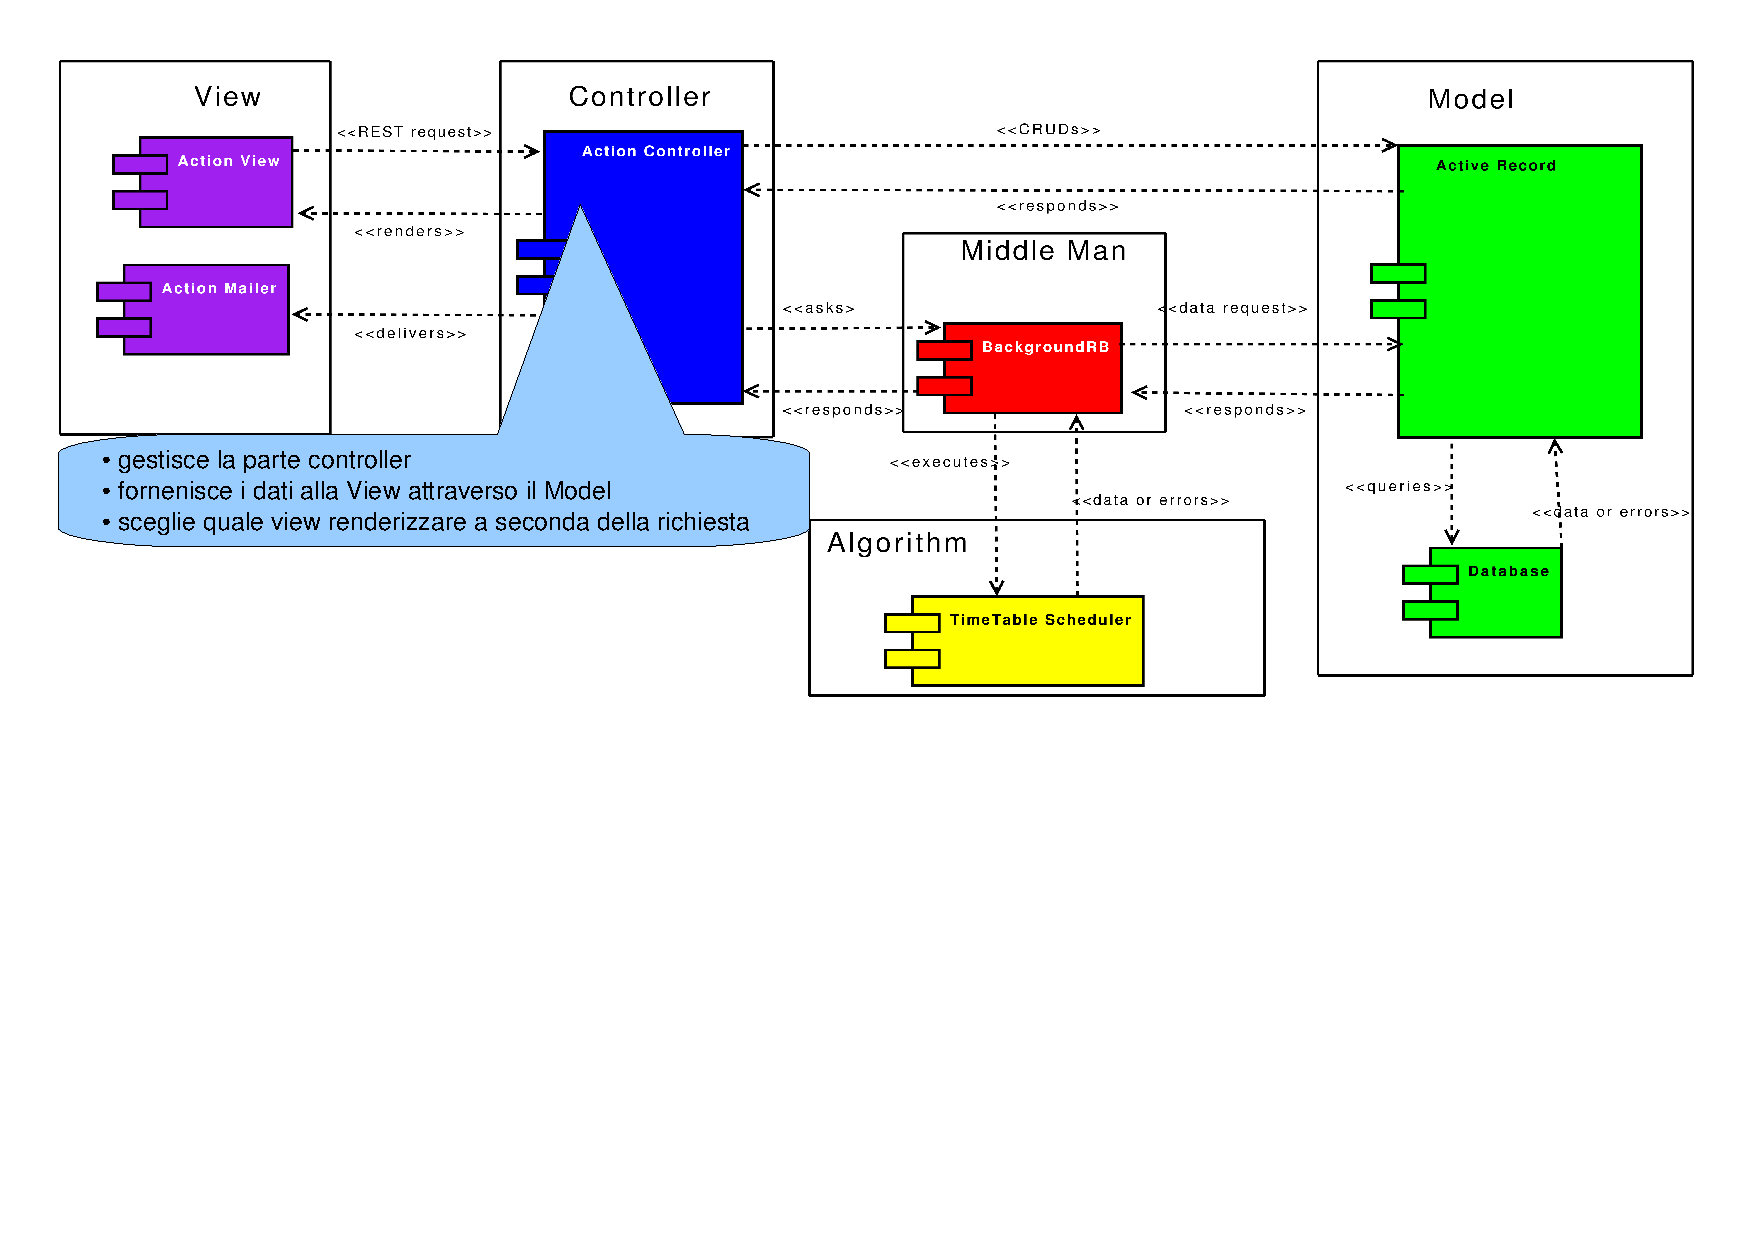
\includegraphics[scale=0.4]{images/diagramma_componenti_controller.pdf}
\end{center}
 \transsplitverticalin
}\frame{
 \frametitle{Specifica tecnica}
 \framesubtitle{Descrizione dei componenti}
\begin{Large}\textbf{Model}\end{Large}
	\begin{center}
 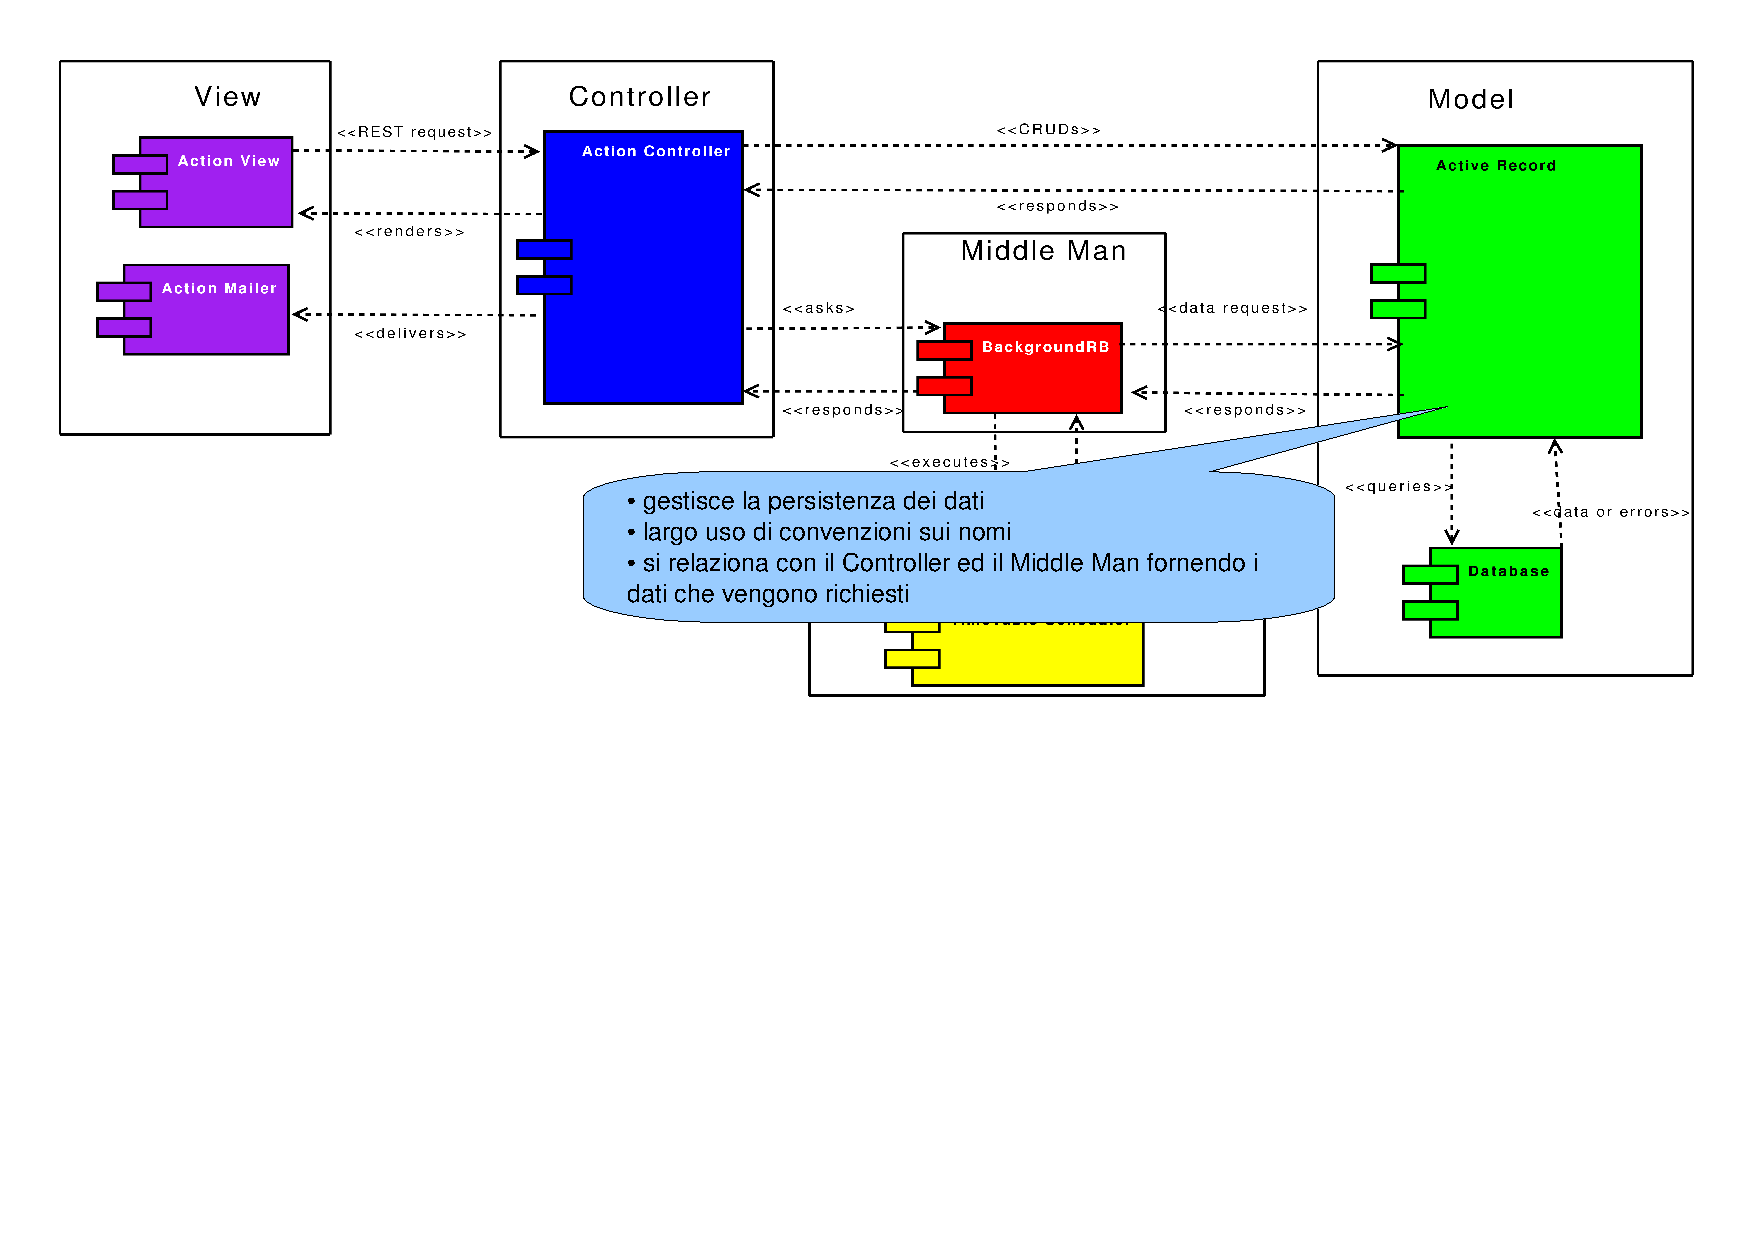
\includegraphics[scale=0.4]{images/diagramma_componenti_model.pdf}
\end{center}
 \transsplitverticalin
}
\frame{
 \frametitle{Specifica tecnica}
 \framesubtitle{Descrizione dei componenti}
\begin{Large}\textbf{MiddleMan}\end{Large}
	\begin{center}
 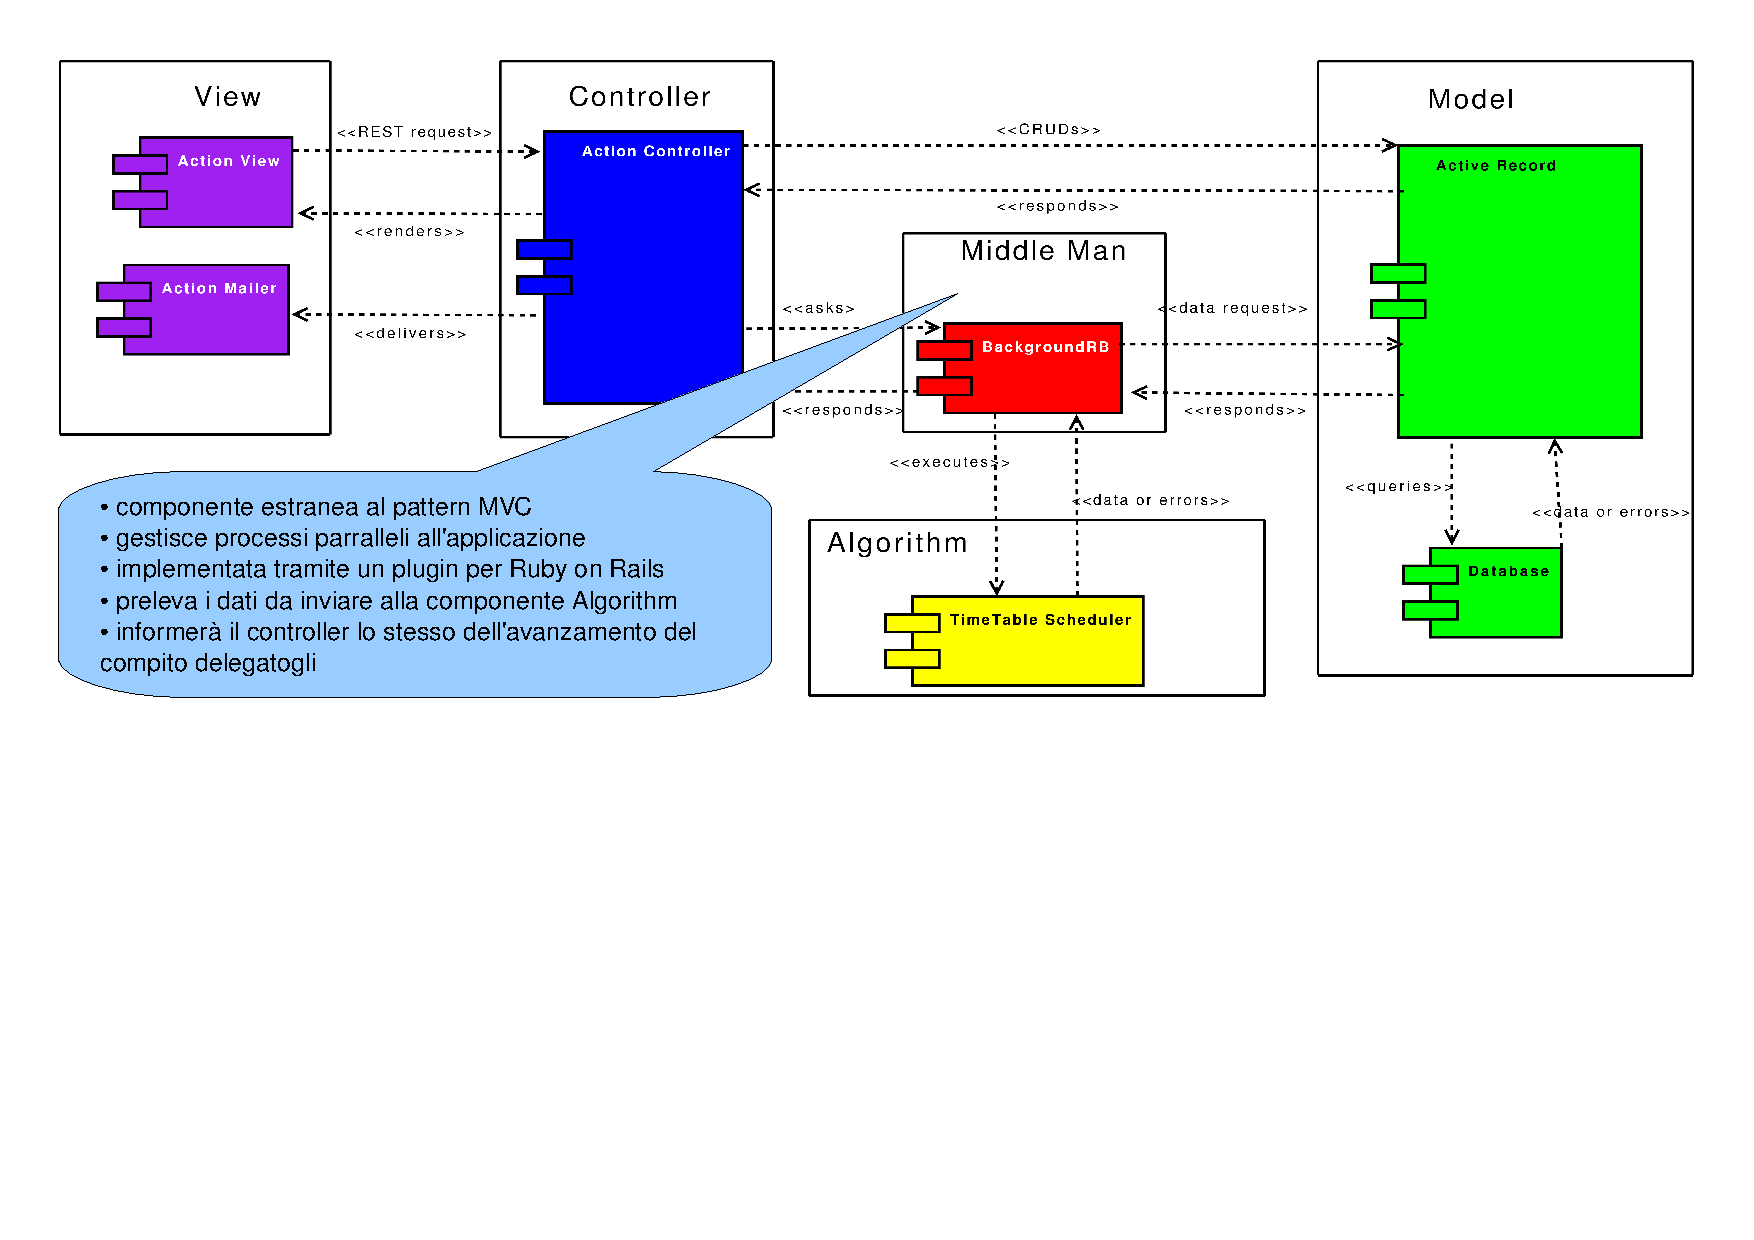
\includegraphics[scale=0.4]{images/diagramma_componenti_middleman.pdf}
\end{center}

 \transsplitverticalin
}
\frame{
 \frametitle{Specifica tecnica}
 \framesubtitle{Descrizione dei componenti}
\begin{Large}\textbf{Algorithm}\end{Large}
	\begin{center}
 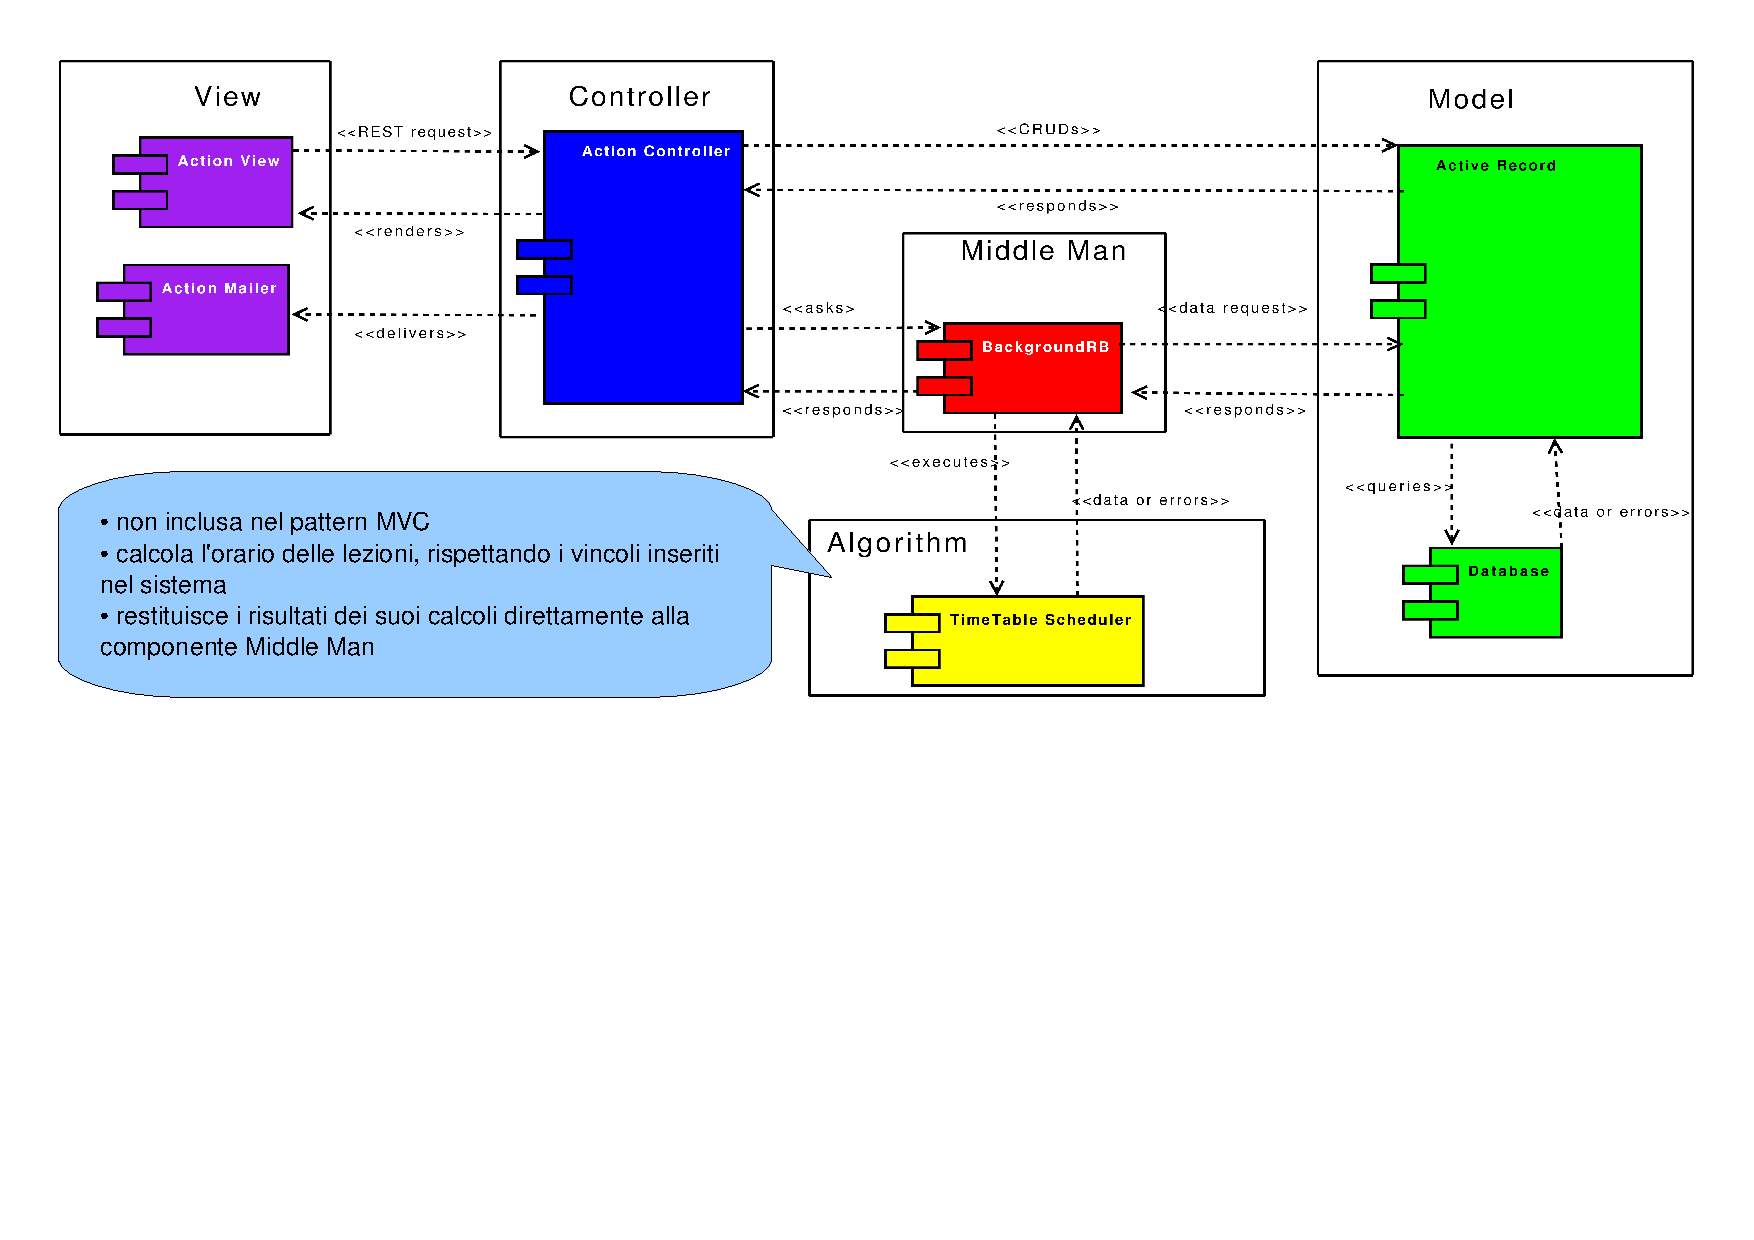
\includegraphics[scale=0.4]{images/diagramma_componenti_algorithm.pdf}
\end{center}
 \transsplitverticalin
}


\subsection{Diagramma delle classi}
\frame{
 \frametitle{Specifica tecnica}
 \framesubtitle{Diagramma delle classi}
 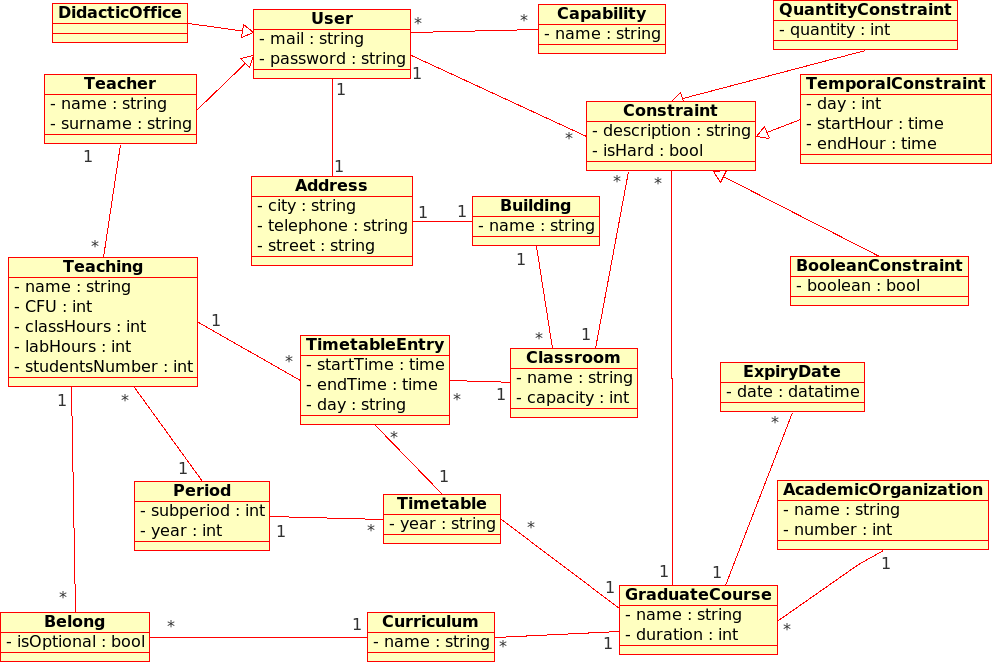
\includegraphics[scale=0.25]{images/diagram_class.png} 
}
\part{Piano di qualifica}
\frame{
	\transsplitverticalin
	\partpage }
\subsection{Aggiornamento piano di qualifica}
\frame{
	\frametitle{Schema generale}
	\transsplitverticalin
	 }\
\end{document}